\section{Funzionalit\`a offerte}
L'applicazione prevede la presenza di un Wallet associato a ciascun tenant, che pu\`o essere ricaricato tramite pagamenti effettuati con \textit{Stripe}.
All'interno del sistema sono previsti dei \textit{workflow}, processi che utilizzano dati provenienti da banche dati esterne per effettuare analisi di vario tipo.
Ogni operazione all'interno del workflow ha un costo, e per ognuna di queste viene scalato un determinato importo in base a un listino prezzi associato al tenant di appartenenza dell'utente.
Quando un'operazione viene inserita nella coda pagamenti, questa viene registrata nel database e il relativo importo viene scalato automaticamente dal Wallet del tenant.\\\\
In questo capitolo ci concentreremo sulle interfacce del Frontend. Per quanto riguarda gli altri requisiti funzionali, verranno discussi in dettaglio nei capitoli successivi.
L'interfaccia prevede la suddivisione in due schermate principali, una per la gestione del Wallet e una per la gestione dei listini prezzi.

\section{Sezione per la gestione del Wallet}
L'utente ha a disposizione una dashboard per monitorare il Wallet del suo tenant di appartenenza in cui pu\`o visualizzare lo storico delle transazioni e ricaricare il Wallet.

\begin{figure}[H]
  \centering
  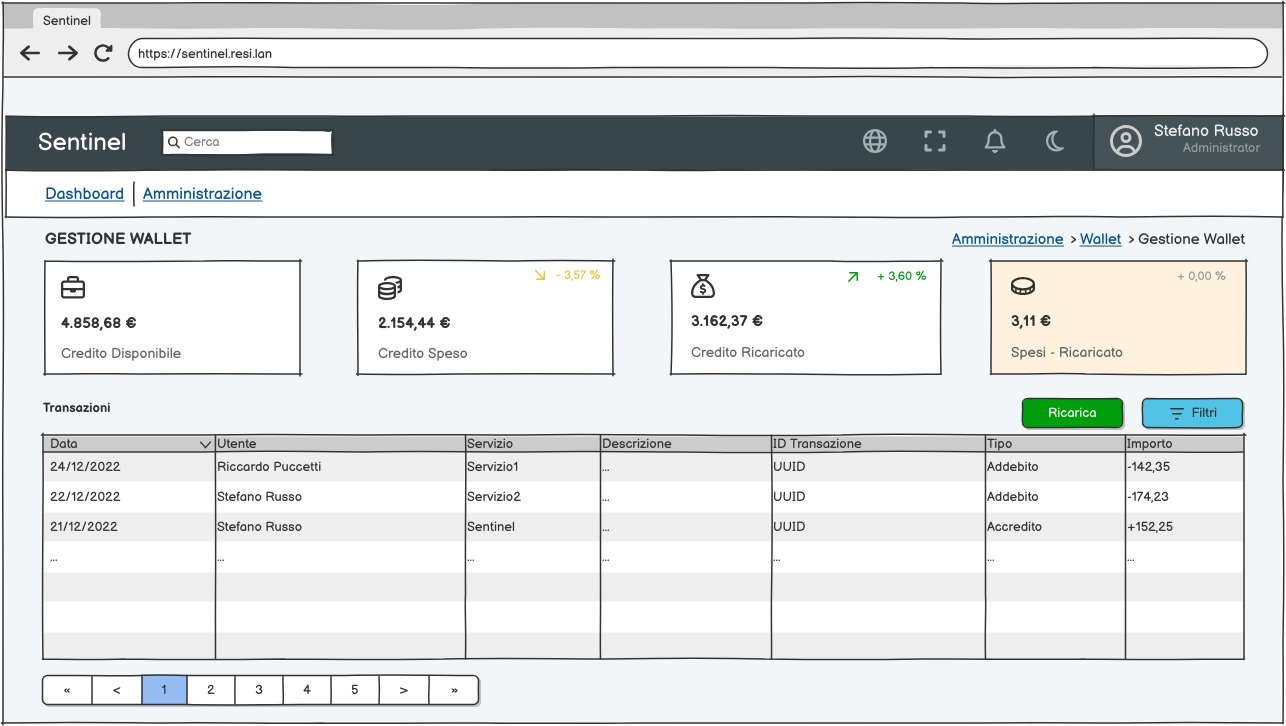
\includegraphics[width=14cm]{images/gestione-wallet/mock-gestione-wallet.png}
  \caption{Wireframe della schermata di Gestione Wallet}
\end{figure}

Nella parte superiore sono presenti dei widget che riportano alcune informazioni in modo da essere facilmente accessibili:
\begin{enumerate}
  \item Credito disponibile
  \item Credito speso  nel mese corrente
  \item Credito depositato nel mese corrente
  \item Differenza tra credito speso e credito depositato nel mese corrente
\end{enumerate}
Gli ultimi tre grafici riportano anche l'andamento rispetto al mese precedente.
\\\\
Il bottone \textit{Ricarica} apre una schermata che permette di caricare un importo arbitrario, con la possibilit\`a di scegliere
dei tagli prestabiliti:

\begin{figure}[H]
  \centering
  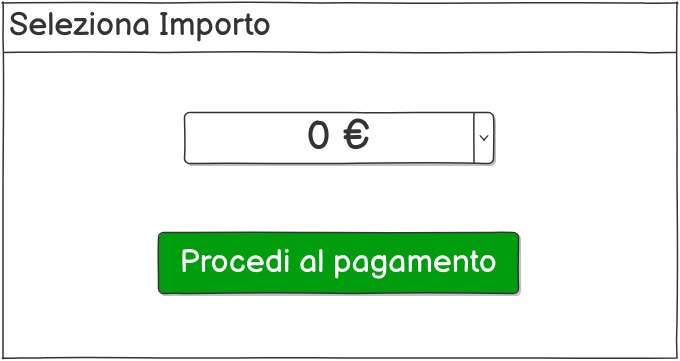
\includegraphics[width=8.5cm]{images/gestione-wallet/mock-seleziona-importo.png}
  \caption{Wireframe della schermata di selezione importo }
\end{figure}
Procedendo al pagamento si conferma l'importo, passando quindi alla schermata di pagamento di Stripe, come illustrato nella figura seguente:

\begin{figure}[H]
  \centering
  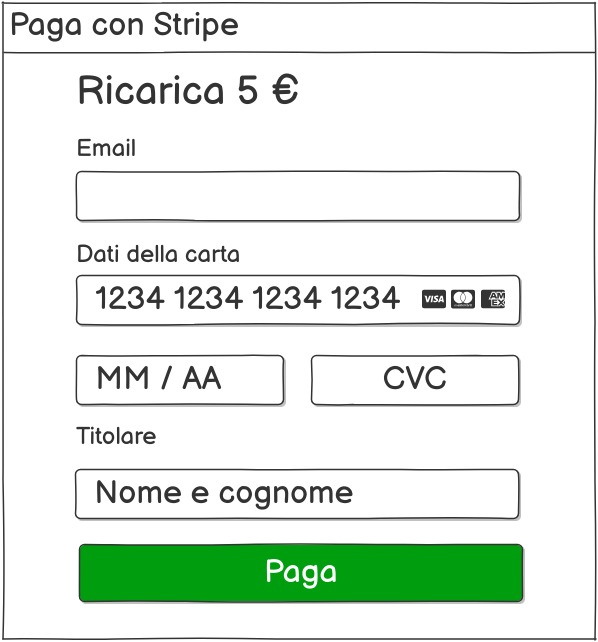
\includegraphics[width=5.5cm]{images/gestione-wallet/mock-stripe.png}
  \caption{Wireframe della schermata di pagamento con Stripe }
\end{figure}

Il bottone \textit{Filtri} apre una schermata laterale dove \`e possibile selezionare le propriet\`a per cui deve essere filtrata la lista delle transazioni.

\begin{figure}[H]
  \centering
  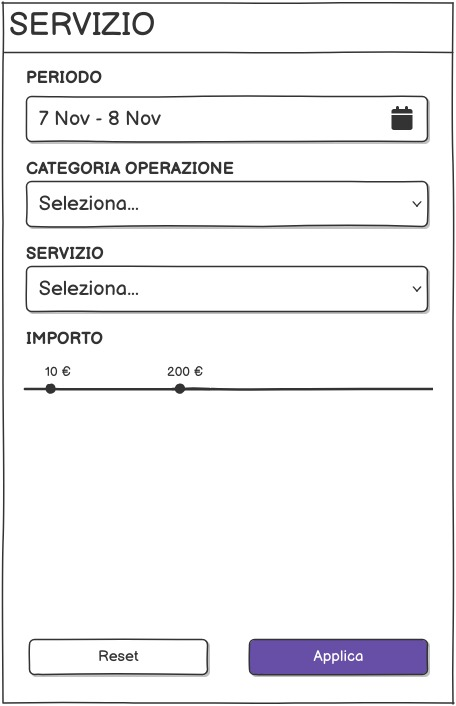
\includegraphics[width=6cm]{images/gestione-wallet/mock-filtri-ricerca.png}
  \caption{Wireframe della schermata dei filtri}
\end{figure}

\section{Sezione per la gestione dei listini prezzi}
